\chapter{Background}
\label{chap:background}

To understand the contribution of this work, we first need to establish the three concepts it builds upon: \emph{term rewriting} as a rule-based process of program transformation, \emph{equality saturation} as a rewrite-based technique for program optimization, and \emph{Knuth–Bendix completion} as a procedure for extending sets of rewrite rules. This chapter provides an informal overview of these topics, focusing on the relevant aspects for program optimization.

\section{Term Rewriting}
\label{sec:term-rewriting}

Term rewriting generally requires two components: a term to be rewritten and a set of directed rewrite rules, also called a \emph{term rewriting system}, or TRS  for short. Figure~\ref{fig:term-rewriting-example} serves as an illustration of the rewriting process. Within figure~\ref{fig:term-rewriting-example}, we find a set of rewrite rules derived from the basic group axioms for addition, as well as a sequence of rewrites, starting at an arithmetic term \emph{t} and ending at term \emph{t'}. Note that some axioms are represented by two rules, one for each direction. 

Performing a rewrite generally requires matching the left-hand side of one of the rules on some subterm of the term to be rewritten and replacing that subterm with the right-hand side of the rule.

\begin{figure}[h]
	\centering
	%====================
	% Left subfigure: Rewrite rules
	%====================
	\begin{subfigure}[c]{0.55\textwidth}
		\vspace*{\fill} % vertical centering
		\raggedright
		R1: $x + 0 \rightarrow x$\\
		R2: $x \rightarrow x + 0$\\
		R3: $0 + x \rightarrow x$\\
		R4: $x \rightarrow 0 + x$\\
		R5: $(x + y) + z \rightarrow x + (y + z)$\\
		R6: $x + (y + z) \rightarrow (x + y) + z$\\
		R7: $-x + x \rightarrow 0$
		\vspace*{\fill}
		\caption{\scriptsize Set of rewrite rules derived from group axioms for addition.}
		\label{fig:term-rewriting-rules}
	\end{subfigure}
	\hfill
	%====================
	% Right subfigure: Rewrite sequence as tree
	%====================
	\begin{subfigure}[c]{0.4\textwidth}
		\centering
		\begin{forest}
			for tree={
				draw,
				rounded corners,
				align=center,
				edge={->},
				parent anchor=south,
				child anchor=north,
				l sep+=8pt,
				s sep+=10pt,
			}
			[$(--a + -a) + a$, no edge
			[$0 + a$, edge label={node[midway,left]{R7}}
			[$a$, edge label={node[midway,left]{R3}}]
			]
			]
			]
		\end{forest}
		\caption{\scriptsize Derivation of $a$ from $(--a + -a) + a$.}
		\label{fig:term-rewriting-tree}
	\end{subfigure}
	
	\caption{Example: term rewriting process for $(--a + -a) + a$ using the group axioms for addition.}
	\label{fig:term-rewriting-example}
\end{figure}

It is important to note that the semantics of the resulting term \emph{t'} remain the same, since the underlying axioms are equalities. Term rewriting, therefore, allows us to find alternative representations of terms while preserving meaning. The number of possible rewrites and, therefore, the number of derivable terms depends on the rule set. In the example shown in figure~\ref{fig:term-rewriting-example}, the rule set contains expansive rules and therefore permits an infinite number of rewrites.

Being able to transform programs into more optimal forms, for some notion of optimality, while preserving meaning, makes term rewriting an interesting approach for program optimization. Crucially, the correctness of the transformations depends solely on the correctness of the employed rewrite rules. 

The connection between term rewriting and computer programs becomes even more apparent when examining functional programming. In other words, a functional program may be viewed as a type of deterministic term rewriting system~\citep{BaaderNipkow1998}. 

This connection with functional programming highlights a limitation when applying term rewriting as a tool for program optimization. While pure functional programming does not rely on mutable state and side effects, programming languages utilizing other paradigms do. As a result, term rewriting may only be applied to those parts of programs that behave like pure functions.

Despite this limitation, term rewriting can still be very effective when optimizing programs, for example, to reduce running time. The technique works particularly well in conjunction with other optimizations such as constant propagation and unreachable code elimination. Consider figure~\ref{fig:term-rewriting-dce}: here, applying the rewrite sequence from figure~\ref{fig:term-rewriting-example} in line two makes it obvious to the compiler that the condition inside the \texttt{if}-statement always holds. As a result, the false branch becomes unreachable and can be removed entirely. 

\begin{figure}[h]
	\centering
	\begin{minipage}{0.48\textwidth}
		\centering
		\textbf{Before Optimization}\\[2pt]
		\begin{lstlisting}[language=C,basicstyle=\footnotesize\ttfamily]
void example(int a) {
  int b = ((-(-a) + -a) + a);
  if ((b - a) == 0) {
  	foo(b);
  } else {
    bar(a);
  }
}
		\end{lstlisting}
	\end{minipage}
	\hfill
	\begin{minipage}{0.48\textwidth}
		\centering
		\textbf{After Optimization}\\[2pt]
		\begin{lstlisting}[language=C,basicstyle=\footnotesize\ttfamily]
void example(int a) {
  int b = a;
  foo(b);
}
		\end{lstlisting}
	\end{minipage}
	\caption{
		Example: unreachable code elimination, enabled by rewriting $(--a + -a) + a$ to $a$.
	}
	\label{fig:term-rewriting-dce}
\end{figure}

\section{Equality Saturation}
\label{sec:equality-saturation}

Equality Saturation (EqSat) is a technique that uses term rewriting to exhaustively derive equivalent terms for one or more input terms. In essence, EqSat applies all applicable rules at every point in a rewrite sequence. To make exhaustive rewriting feasible, even for TRS that permit an infinite number of derivations, such as in figure~\ref{fig:term-rewriting-example}, EqSat uses a special data structure called an e-graph to represent terms compactly.

An e-graph contains e-nodes and e-classes, with the former being term symbols and the latter being equivalence classes that each contain the set of root symbols of equivalent terms. Applying rewrite rules grows the e-graph by adding new nodes, and a rebuilding step ensures that equivalent terms are part of the same e-class. 

A major advantage of this data structure is that expansive patterns, such as addition of 0 in arithmetic, don’t grow the graph infinitely. As a result, the e-graph may reach a fixpoint, at which additional iterations of rule applications don’t change the graph anymore. At this point, saturation is reached, and the optimal term can be extracted from the graph~\citep{Willsey_2021}.

Figure~\ref{fig:e-graph-sub1} shows the familiar term $(--a + -a) + a$ as an e-graph. The symbol 'root+' refers to the second addition in the term, but is marked with 'root', so it is easier to identify as the root symbol.

Further, we see that all nodes have their own equivalence classes, indicated by the dashed boxes around them. This changes when we apply associativity as a rule. In figure~\ref{fig:e-graph-sub2} we see that 'root+' now shares an equivalence class with the root symbol of the associative counterpart $(--a + (-a + a))$.

After applying a total of four rules, we end up at figure~\ref{fig:e-graph-sub4}. It is important to note that we applied rules selectively and that more rules could be applied after every step. In practice, this would happen during EqSat; however, the resulting e-graph would quickly become too complex to serve an illustrative purpose.

\begin{figure}[h]
	\centering
	\begin{subfigure}[t]{0.23\textwidth}
		\centering
		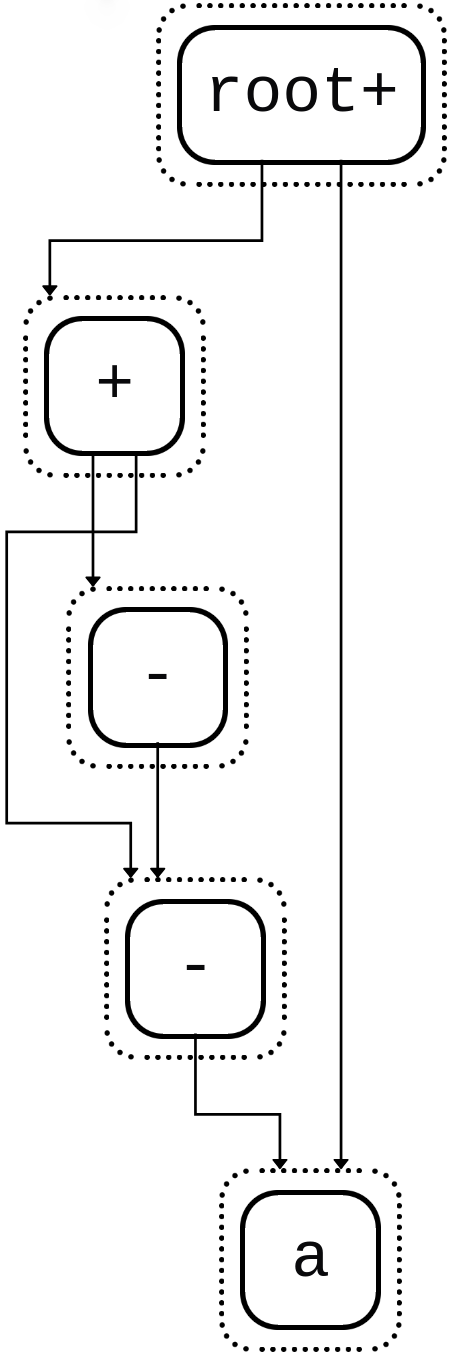
\includegraphics[width=1.4\linewidth,height=1.4\linewidth,keepaspectratio=true]{img/e_graph1.png}
		\caption{\scriptsize Term $(--a + -a) + a$}
		\label{fig:e-graph-sub1}
	\end{subfigure}
	\hfill
	\begin{subfigure}[t]{0.27\textwidth}
		\centering
		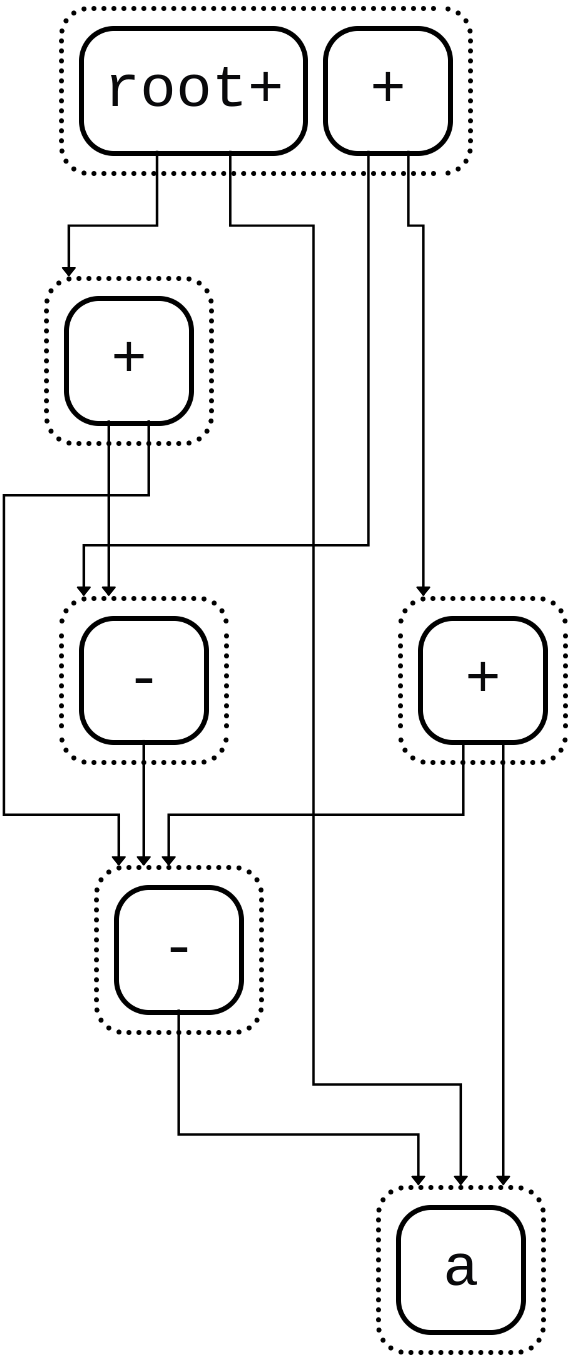
\includegraphics[width=1.19\textwidth,height=1.19\textwidth,keepaspectratio=true]{img/e_graph2.png}
		\caption{\scriptsize After applying\\$(X + Y) + Z \to X + (Y + Z)$}
		\label{fig:e-graph-sub2}
	\end{subfigure}
	\hfill
	\begin{subfigure}[t]{0.23\textwidth}
		\centering
		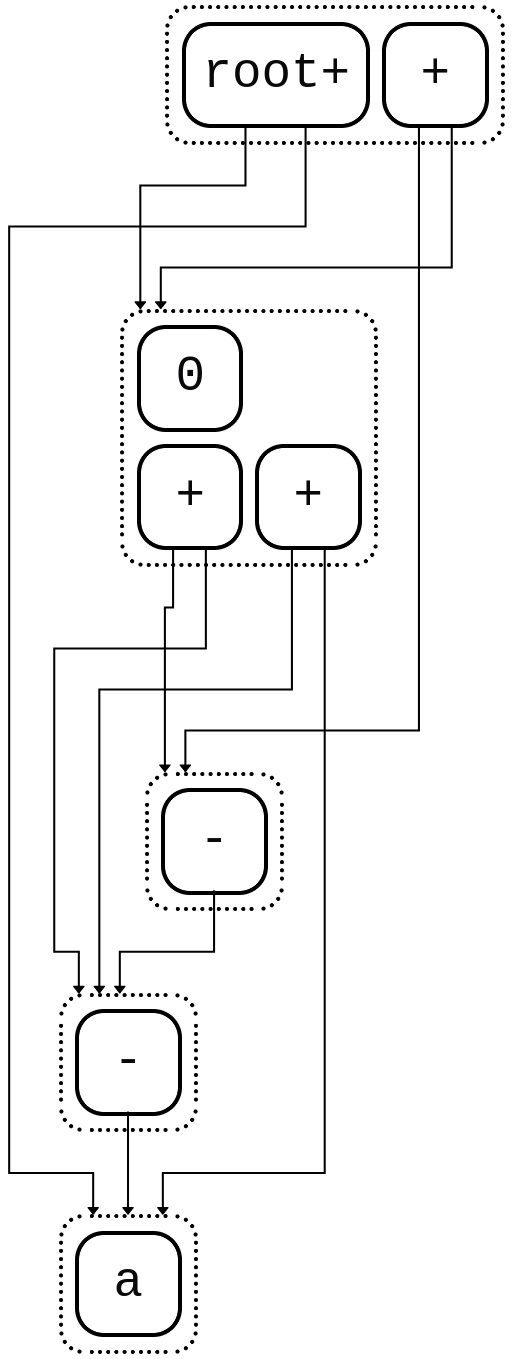
\includegraphics[width=1.4\linewidth,height=1.4\linewidth,keepaspectratio=true]{img/e_graph3.png}
		\caption{\scriptsize After applying\\$-X + X \to 0$}
		\label{fig:e-graph-sub3}
	\end{subfigure}
	\hfill
	\begin{subfigure}[t]{0.23\textwidth}
		\centering
		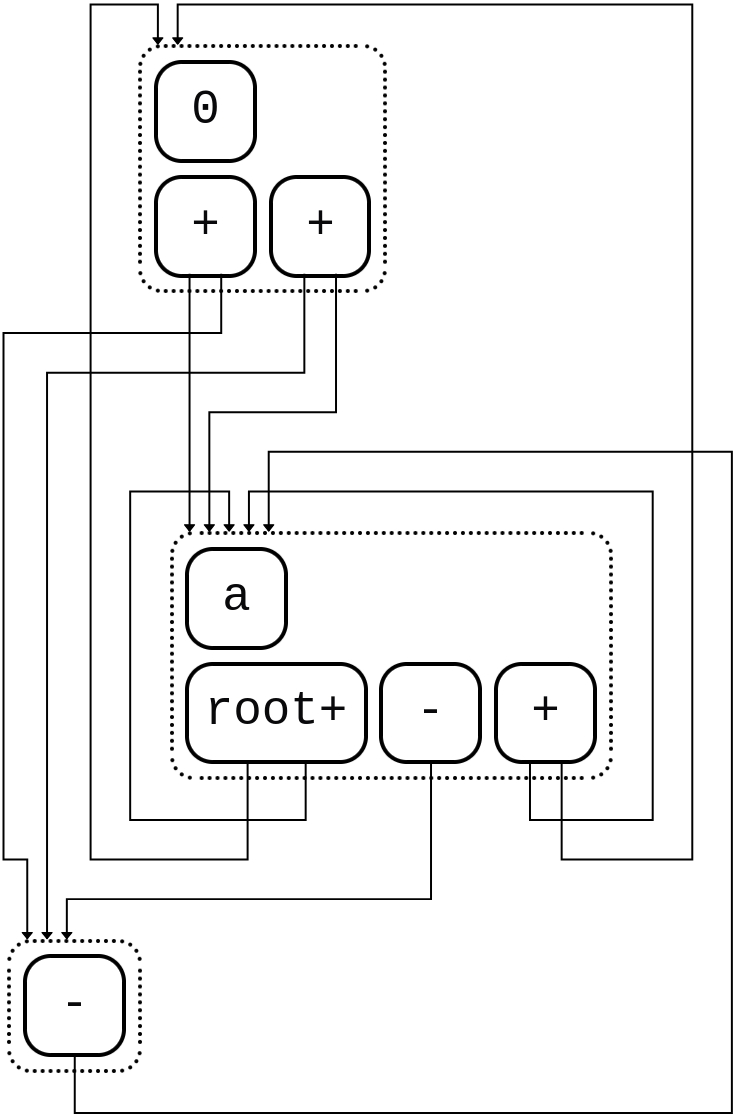
\includegraphics[width=1.4\linewidth,height=1.4\linewidth,keepaspectratio=true]{img/e_graph4.png}
		\caption{\scriptsize After applying\\$0 + X \to X$ and\\$X + 0 \to X$}
		\label{fig:e-graph-sub4}
	\end{subfigure}
	\caption{Example: representation of $(--a + -a) + a$ as an e-graph and application of four rewrite rules. e-nodes in graph shown as solid boxes, e-classes as dashed boxes.}
	\label{fig:e-graph-example}
\end{figure}

There are multiple options for terminating EqSat. Ideally, the process ends on saturation of the e-graph. That is, the procedure runs until additional rule applications do not change the e-graph anymore. In this case, EqSat found all possible derivations. 

In practice, saturation is uncommon due to EqSat being resource-intensive. Rules such as associativity and commutativity in particular increase graph size exponentially~\citep{zhang2023}, making it likely that for sufficiently complex terms and rule sets, memory becomes a limiting factor. Therefore, in many cases, termination of EqSat depends on specified resource limits.

A key advantage offered by EqSat is that the process of finding terms happens independently of the rewrite goal. After termination, one can extract the desired term by using a cost function. For this, consider again figure~\ref{fig:e-graph-sub4}. By locating the equivalence class containing 'root+', we find the roots of all terms equivalent to our original term. The set containing all of these terms consists of all paths from the root nodes to leaves. It is now easy to verify that the rewrite from figure~\ref{fig:term-rewriting-example} contained in the e-graph, by confirming that the node 'a' is inside the e-class of 'root+'. Extracting the optimal term from an e-graph is in itself a challenge and subject of ongoing research~\citep{yin2025eboostboostedegraphextraction}.

\section{Knuth-Bendix Completion}
\label{sec:knuth-bendix-completion}

Knuth-Bendix completion (KBC), unlike EqSat, is a rewrite-based technique that has not seen significant attention in the context of program optimization. Instead, it is primarily used in automated theorem proving. When trying to prove the equivalence of two terms \emph{s} and \emph{t} using term rewriting, we need to show that we can either rewrite \emph{s} to \emph{t}, \emph{t} to \emph{s}, or \emph{s} and \emph{t} to a third term \emph{u}. A KBC-based proof uses the latter approach, although $\emph{u} = \emph{t}$ or $\emph{u} = \emph{s}$ may hold.

The term \emph{u} used in such a proof is known as the normal form of the set of equivalent terms it belongs to. If \emph{s} and \emph{t} are equal, they must share the same normal form. While this normal form is not explicitly known beforehand, it is uniquely determined as it is the smallest term in its equivalence class according to some ordering. We will refer to this ordering as the \emph{Knuth-Bendix ordering} (KBO). There are a number of formal requirements for an ordering to be considered a KBO, which~\cite{BaaderNipkow1998} elaborate on in detail. Most importantly, KBO is a well-founded simplification order. This implies that for all equivalence classes of ground terms, i.e., terms that do not contain variables, there exists a unique smallest element. 

To understand how KBC works in more detail, we will reformulate the example from figure~\ref{fig:term-rewriting-example} as a proof goal. For this let the $\emph{t} = (--a + -a) + a$ and $\emph{s} = a$. In this case, it is obvious that $a$ is the normal form of \emph{t}. Therefore, one possible proof consists of performing the sequence of rewrites from figure~\ref{fig:term-rewriting-example}. The first step for proving this equality using KBC requires replacing the original set of rewrite rules with a set in which, for all rules, the left-hand side is larger under KBO than the right-hand side. This ensures that whenever a rewrite is applied, the term becomes smaller and therefore closer to its normal form.

For the axioms of addition, the directions for all but two axioms coincide with intuition. That is, if a term has fewer symbols, it is smaller. This is reflected by the usage of a weight function in KBO. In the case of associativity and commutativity, both sides of the axiom share the same symbols and therefore their weight is the same. In such a case, KBO orders terms lexicographically. In the case of associativity this means $(X + Y) + Z >_{KBO} X + (Y + Z)$ since $(X + Y) >_{KBO} X$. In the case of commutativity, this method also fails, which is why basic variants of KBC fail when encountering such an axiom. Extensions of the basic KBC algorithm solve this issue by keeping unorderable rules unordered until they are instantiated. Those variants are known as \emph{unfailing} KBC~\citep{10.1093/comjnl/34.1.2} and will be referred to simply as KBC throughout this paper.

After orienting the initial set of axioms, we can already try applying the rules. Figure~\ref{fig:kbc-example} shows the directed rules, as well as a rewrite sequence derived using said rules. Note that the derived sequence differs from figure~\ref{fig:term-rewriting-example} in the first step and as a result does not end with the normal form $a$, but instead with $--a$. 

\begin{figure}[h]
	\centering
	% First subfigure: left-aligned, vertically centered
	\hfill
	\begin{subfigure}[c]{0.55\textwidth}
		\vspace*{\fill} % allow vertical centering
		R1: $0 + X \rightarrow X$\\
		R2: $X + 0 \rightarrow X$\\
		R3: $-X + X \rightarrow 0$\\
		R4: $(X +Y) + Z \rightarrow X + (Y + Z)$
		\vspace*{\fill}
		\caption{\scriptsize Subset of group axioms for addition, directed using KBO}
		\label{fig:kbc-sub1}
	\end{subfigure}
	\hfill
	% Second subfigure: forest diagram
	\begin{subfigure}[c]{0.4\textwidth}
		\centering
		\begin{forest}
			for tree={
				draw,
				rounded corners,
				align=center,
				edge={->},
				parent anchor=south,
				child anchor=north,
				l sep+=8pt,
				s sep+=10pt,
			}
			[$(--a + -a) + a$, no edge,
			[$--a + ((-a) + a)$, edge label={node[midway,left]{R4}}
			[$--a + 0$, edge label={node[midway,left]{R3}}
			[$--a$, edge label={node[midway,left]{R2}}]
			]
			]
			]
		\end{forest}
		\caption{\scriptsize Derivation of $--a$ from $(--a + -a) + a$}
		\label{fig:kbc-sub2}
	\end{subfigure}
	
	\caption{Example: derivation of $--a$ from $(--a + -a) + a$ using a subset of the group axioms for addition, directed according to KBO.}
	\label{fig:kbc-example}
\end{figure}

\FloatBarrier
At this point, no more rules can be applied. While $--a$ is smaller than $(--a + -a) + a$, we still need to prove $--a = a$. To do this, however, the current rule set is insufficient. In a case like this, the KBC algorithm can be used to generate new rewrite rules.

To derive new rewrite rules, KBC uses a concept called \emph{superposition}. For this, the left-hand side of a rewrite rule is matched on the left-hand side of another rule. If a match exists for two rules, a new term can be constructed through unification. 

This term can then be rewritten using the two rules it was constructed with. The result of these rewrites is a pair of terms, which must be equal, since they were derived from the same term using existing rewrite rules. Such a pair is called a \emph{critical pair}. If the critical pair is not trivially equal after normalizing, i.e, applying the existing rewrite rules, it is certain that the terms are equal but cannot be proven equal using the existing rules. Therefore, the critical pair is ordered, using KBO, and introduced as a new rule~\citep{10.1093/comjnl/34.1.2}.

Figure~\ref{fig:superpos-example} illustrates this process, by deriving the rule $--a \to a$ using superposition of rules from figure~\ref{fig:kbc-sub1}.

\begin{figure}[h]
	\centering
	
	%====================
	%  Main Subfigure (a,b)
	%====================
	\begin{subfigure}[c]{\textwidth}
		\centering
		
		%--- (a) Rules
		\begin{minipage}[c]{0.45\textwidth}
			\raggedright
			Rewrite rules:\\[3pt]
			R1: $0 + X \rightarrow X$\\
			R2: $X + 0 \rightarrow X$\\
			R3: $\textcolor{red}{-X + X} \rightarrow 0$\\
			R4: $(\textcolor{red}{X + Y})\textcolor{blue}{ + Z} \rightarrow X + (Y + Z)$\\
			\textcolor{gray}{R5: $-X + (X + Z) \rightarrow Z$}
		\end{minipage}
		\hfill
		%--- (b) Forest diagram
		\begin{minipage}[c]{0.45\textwidth}
			\centering
			\begin{forest}
				for tree={
					draw,
					rounded corners,
					align=center,
					edge={->},
					parent anchor=south,
					child anchor=north,
					l sep+=15pt,
					s sep+=10pt
				}
				[$(\textcolor{red}{-X + X}) \textcolor{blue}{+ Z}$
				[$-X + (X + Z)$, edge label={node[midway, left]{R4}}, name=A]
				[$0 + Z$, edge label={node[midway, right]{R3}}
				[$Z$, edge label={node[midway, right]{R1}}, name=B]
				]
				]
				{\draw[->, dashed] (A) -- (B) node[midway, right]{R5};}
			\end{forest}
		\end{minipage}
		
		\caption{\scriptsize Derivation of $-X + (X + Z) \rightarrow Z$ by superposition of R3 and R4.}
		\label{fig:superpos-ab}
	\end{subfigure}
	
	\vspace{2em}
	
	%====================
	%  Main Subfigure (c,d)
	%====================
	\begin{subfigure}[c]{\textwidth}
		\centering
		
		%--- (c) Rules (repeat or variant)
		\begin{minipage}[c]{0.45\textwidth}
			\raggedright
			Rewrite rules:\\[3pt]
			R1: $0 + X \rightarrow X$\\
			R2: $X + 0 \rightarrow X$\\
			R3: $\textcolor{red}{-X + X} \rightarrow 0$\\
			R4: $(X + Y) + Z \rightarrow X + (Y + Z)$\\
			R5: $\textcolor{blue}{-X +} (\textcolor{red}{X + Z}) \rightarrow Z$\\
			\textcolor{gray}{R6: $--X \rightarrow X$}
		\end{minipage}
		\hfill
		%--- (d) Forest diagram
		\begin{minipage}[c]{0.45\textwidth}
			\centering
			\begin{forest}
				for tree={
					draw,                   % draw boxes around nodes
					rounded corners,        % rounded node corners
					align=center,           % center text
					edge={->},              % arrows for edges
					parent anchor=south,    % connect edges from bottom of parent
					child anchor=north,     % connect edges to top of child
					l sep+=15pt,            % increase level separation
					s sep+=15pt             % increase sibling separation
				}
				[$\textcolor{blue}{--X +} (\textcolor{red}{-X + X})$
				[$--X + 0$, edge label={node[midway, left]{R3}}
				[$--X$, edge label={node[midway, left]{R2}}, name=A]]
				[$X$, before drawing tree={y-=2.3cm}, edge label={node[midway, right]{R5}}, name=B]]
				]
				\draw[->, dashed] (A) -- (B)  node[midway, above]{R6};
			\end{forest}
		\end{minipage}
		
		\caption{\scriptsize Derivation of $--X \rightarrow X$ by superposition of R3 and R5.}
		\label{fig:superpos-cd}
	\end{subfigure}
	
	%====================
	%  Main Figure Caption
	%====================
	\caption{
		Example: derivation of rules $-X + (X + Z) \rightarrow Z$ and $--X \rightarrow X$ using superposition. Matched subterms are marked red, derived rules are marked gray.
	}
	\label{fig:superpos-example}
\end{figure}

The rule derived in figure~\ref{fig:superpos-cd} now enables a rewrite from $--a$ to $a$. This derivation step completes the proof from figure~\ref{fig:kbc-example}. In fact, with the extended rule set, proving $(--a + -a) + a = a$ becomes trivial, since matching rules can be applied in an arbitrary order to reach the normal form. By running KBC sufficiently long, i.e., continuously generating more rewrite rules, this eventually holds for all pairs of terms that are equivalent with respect to the underlying axioms.

A TRS with this property is called a \emph{confluent} TRS. Formally, confluence denotes that any two terms that can be derived from the same term can be simplified to a common descendant. It directly follows, then, that to find the normal form for a given term, it suffices to apply rewrite rules exhaustively in any order.

Whether a finite confluent TRS exists depends on the given set of axioms. If it does exist, KBC will eventually stop generating critical pairs that, after normalization, are not trivially equal. At this point, the algorithm terminates. If no finite confluent TRS exists, KBC diverges. When trying to prove theorems, divergence turns KBC into a semi-decision procedure~\citep{10.1093/comjnl/34.1.2}. That is, any two terms that are in fact equal will eventually be proven to be equal.